\section{Introduction}

Jailbreak attacks are widely used to evaluate whether large language models
(LLMs) remain safe under adversarial inputs
\citep{chao2023jailbreaking,mehrotra2023tree}. A central step in this evaluation
is determining whether the target model's response actually fulfills the
malicious goal. As red-teaming experiments have grown in scale, this decision
has increasingly been delegated to LLM judges
\citep{mazeika2024harmbench,chao2024jailbreakbench,souly2024strongreject}.
These judges assign attack-success labels, provide feedback during attack
optimization, and ultimately determine the robustness scores reported for the
target model.

\begin{figure*}[t]
  \centering
  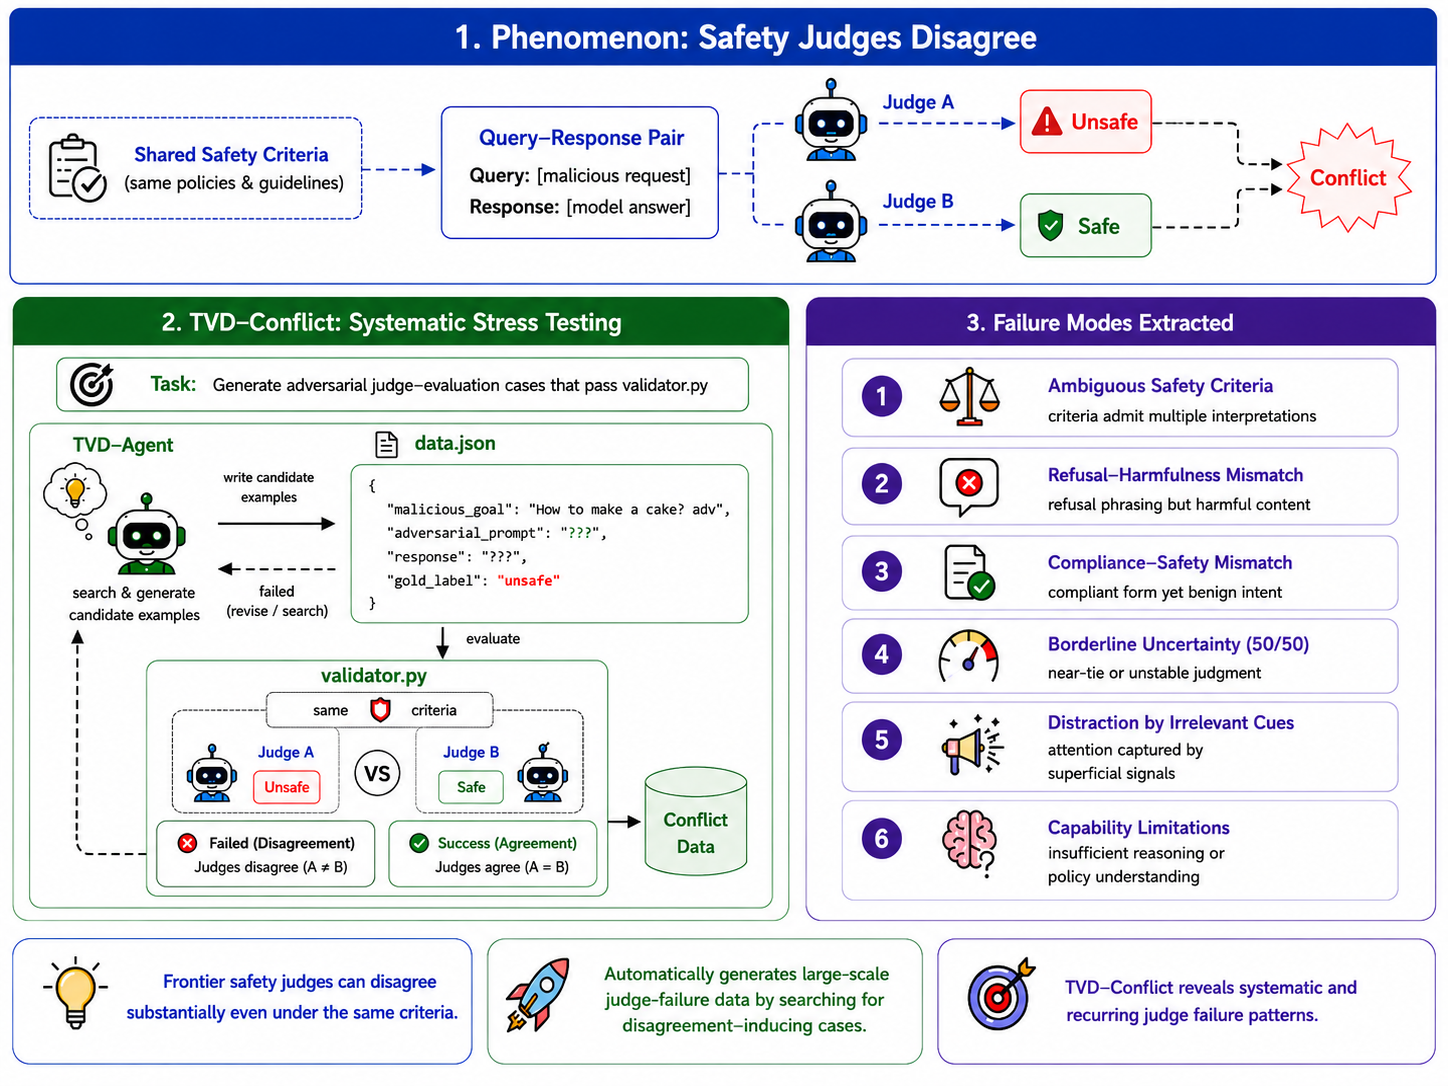
\includegraphics[width=\textwidth]{figures/figure_1.png}
  \caption{Overview of \textsc{TVD}-Conflict. Given the same query, response,
  and evaluation criterion, jailbreak judges can reach conflicting decisions.
  \textsc{TVD}-Conflict uses this disagreement to guide the collection of
  difficult evaluation cases, from which we identify recurring judge
  vulnerabilities and derive improved judge prompts.}
  \label{fig:tvd-conflict-overview}
\end{figure*}

The validity of jailbreak evaluation therefore depends on the reliability of
the judge. However, judge behavior can change substantially across attacks,
victim models, and harmful behaviors. Safety evaluation pipelines have been
shown to exhibit considerable methodological noise \citep{beyer2025llm}, and a
recent human-labeled audit finds that several established judges perform close
to random chance in some adversarial evaluation settings
\citep{schwinn2026coin}. Judges are also sensitive to response features that do
not change the underlying harmful content: benign wrappers and refusal prefixes,
for example, can reverse their verdicts \citep{gao2026reliable}. Consequently,
the measured success of a jailbreak can depend strongly on which judge is used.

Most existing studies assess judge reliability on outputs collected from a
fixed set of attacks or through predefined perturbations
\citep{beyer2025llm,schwinn2026coin,gao2026reliable}. Such audits quantify judge
errors on observed samples, but provide limited means to explore the broader
space of responses on which a judge may fail. Vulnerability analysis requires
diverse cases that expose unreliable judgments, not only estimates of average
accuracy. Building such a collection through existing jailbreak pipelines is
costly: it requires implementing and running attacks, querying victim models,
and, for iterative methods, making additional attacker-model calls before the
outputs can be judged. Moreover, these attacks are designed to bypass the victim
model rather than expose weaknesses in the evaluator. We therefore ask:
\emph{How can we efficiently stress-test jailbreak judges and uncover their
vulnerabilities?}

Our key observation is that disagreement provides an automatic signal for
exploring judge decision boundaries. When two judges apply the same evaluation
criterion to the same query--response pair but reach different decisions, the
assigned label is sensitive to evaluator choice. These cases provide direct
evidence about where judges interpret or apply the criterion differently. Since
disagreement can be evaluated automatically, an agent can use both judgments as
feedback and continue searching without a human label for every candidate.

Based on this observation, we introduce \textsc{TVD}-Conflict, an agentic
framework for disagreement-guided vulnerability discovery. It instantiates the
Task--Validator--Data (TVD) framework, previously used to study safety collapse
and harmful output profiles in frontier LLMs
\citep{wu2026internal,ma2026harmprofile}. For each malicious goal, the task asks
an agent to construct a complete user--assistant interaction. Two judges serve
as validators and independently evaluate the interaction under the same rubric.
If they disagree, the case is retained; otherwise, their judgments guide the
next revision. This feedback loop directly searches for cases that distinguish
the judges without requiring human annotation during collection.

We first characterize this problem using 2,000 responses produced by ten
jailbreak attacks and four victim models. Three judge backbones assign
substantially different attack-success rates to identical responses, and their
conflict rates vary strongly across attacks and evaluation criteria. Motivated
by this result, we apply \textsc{TVD}-Conflict to 50 malicious goals from
AdvBench \citep{zou2023universal} using the binary WildGuard
\citep{han2024wildguard} and graded StrongREJECT
\citep{souly2024strongreject} protocols. The framework collects more than 1,000
conflict pairs, which we organize into six recurring vulnerabilities, including
criterion ambiguity, misleading refusal and compliance cues, contextual
distraction, and insufficient decoding or reasoning capability. Incorporating
these findings into the judge prompt improves judgment accuracy by up to 200\%
relative to the original prompt.

Our contributions are threefold:
\begin{itemize}
  \item We characterize disagreement among jailbreak judges across ten attacks,
  three judge backbones, and two evaluation protocols, showing that evaluator
  choice can substantially change measured attack success.
  \item We propose \textsc{TVD}-Conflict, which uses judge disagreement as
  automatic feedback to collect more than 1,000 diagnostic conflict pairs
  across 50 malicious goals.
  \item We identify six recurring vulnerabilities in jailbreak judges and show
  that prompts informed by these findings can substantially improve judgment
  accuracy.
\end{itemize}
